nEste capítulo apresenta, inicialmente, os diferentes tipos de escalonadores, citando as várias áreas em que a atividade de escalonamento ocorre. Em seguida apresenta a definição do problema de escalonamento que este trabalho busca resolver. Em sequência, é discorrido sobre trabalhos relacionados para então apresentar o algoritmo de escalonamento proposto.

\section{Definição}

O escalonamento é um problema clássico da computação que surgiu junto com os sistemas operacionais multitarefas. A sua complexidade é considerada NP-difícil\cite{ULLMAN1975384}, porém isso não impediu a evolução dos sistemas operacionais, cujos escalonadores são desenvolvidos com objetivos e metodologias diferentes para alcançarem uma boa performance. De qualquer forma, um problema que todos os sistemas operacionais multitarefa buscam resolver é o \textit{starvation}, que é quando um processo/\textit{thread} fica esperando indefinidamente por um recurso, que pode ser, inclusive, a \acrshort{CPU} \cite{TANEMBAUM_SO}.

Escalonadores podem ser categorizados de várias formas, com base nas funcionalidades que possuem. Assim, uma importante questão é definir qual é a unidade escalonada, podendo ser\cite{TANEMBAUM_SO}:

	\begin{itemize}
		\item processos, \textit{threads} para serem executados;
		\item \textit{jobs} para serem excecutados na nuvem;
		\item páginas da memória \acrfull{RAM} para \textit{swapping};
		\item pacotes para serem transmitidos pela rede;
		\item requisições de leitura/escrita em memória secundária.
	\end{itemize}

	Além da unidade que é escalonada, outras características que ajudam a definir um escalonador é se ele permite que tarefas sejam interrompidas para que outras possa ser executadas, funcionalidade conhecida como preempção. Além disso, o escalonador pode ou não ser capaz de definir prioridade diferentes para cada um dos objetos que está sendo escalonado, e/ou dá suporte para processos que podem requisitar urgência para sua execução, conhecidos como processos de tempo-real\cite{TANEMBAUM_SO}.

%	\item \textbf{Suporte para preempção}: Se permite interrupção de uma tarefa em execução para atender outras;
%	\item \textbf{Suporte para prioridade}: Se permite que priorização entre as tarefas que serão escalonadas;
%	\item \textbf{Suporte para para tempo-real}: Se permite que requerem execução constante tenham esse requisito atendido.
%\end{itemize}


O problema do escalonamento é o método pelo qual o trabalho, definido por algum conjunto de características (como duração e requisitos), é atribuído aos recursos que são capazes de completá-lo. %Por mais que exista a dificuldade teórica \cite{ULLMAN1975384}, isso não impediu a evolução dos sistemas operacionais, os quais são capazes de fazer escalonamento de vários processos.

Atualmente, as \acrshort{CPU}s possuem vários núcleos, e são capazes de ter mais de um contexto carregado por núcleo (vide Ryzen™ Threadripper™\cite{Ryzen}). O que faz com que seja necessário que o processo de escalonamento leve em consideração como o mesmo será distribuído (ou não) entre os núcleos.

A atividade de escalonamento pode ser otimizada para vários objetivos, entre os quais é possível citar\cite{TANEMBAUM_SO}:
\begin{itemize}
	\item Maximinizar quantidade de trabalho realizada por unidade de tempo;
	\item Minimizar tempo no qual trabalhos ficam esperando para serem executados;
	\item Minimizar tempo entre um conjunto de trabalhos estar pronto para ser executado até o fim da execução do conjunto (\textit{timespan});
	\item Distribuir de forma justa o tempo que cada um dos trabalhos terá de uso de um recurso escasso.
\end{itemize}

Esses objetivos são, às vezes, contraditórios. Na prática, prioriza-se um conjunto de métricas como base para otimização. Por exemplo, o GNU/Linux utiliza o \acrfull{CFS}, que se baseia no algoritmo \textit{Fair queuing}. Como o nome já diz, o foco desse escalonador está em ser justo. Internamente, utiliza-se uma árvore rubro-negra indexada pelo tempo gasto no processador. Para ser justo, o tempo máximo de cada processo na \acrshort{CPU} é o quociente do tempo que o processo ficou aguardando para ser executado pelo número total de processos.

\section{Escalonamento em Nuvens Computacionais}
O escalonamento em nuvens computacionais podem ocorrer em vários contextos e com focos distintos \cite{Zhan:2015:CCR:2775083.2788397}, como podemos ver na Figura \ref{EscalonamentoStack}. O escalonamento ocorre geralmente de uma camada inferior para uma camada superior da pilha de serviços da nuvem, mas no caso de federações horizontais o escalonamento pode ocorrer numa mesma camada. 

No contexto da camada de virtualização o objetivo do escalonamento é mapear recursos virtualizados a recursos físicos, podendo focar no balanço de carga, ou seja, distribuir o máximo possível o processamento entre os recursos físicos disponíveis para evitar que sobrecargas ocorram enquanto outra parte dos recursos estão ociosos, na conservação de energia, buscando alocar no mínimo de máquinas disponíveis, para reduzir custo energético ou então focar no custo-benefício, que, é parecido com o foco em conservação de energia, porém leva em consideração também outros fatores que podem interferir no custo, como a localização do equipamento, como o custo do próprio equipamento, histórico de utilização do usuário (se o mesmo costuma subutilizar os recursos ou não), entre outros fatores \cite{Zhan:2015:CCR:2775083.2788397}.

\begin{figure}[htbp]
	%	\centerline{\includegraphics[scale=0.04]{img/EscalonadorProposto.png}}
	\centerline{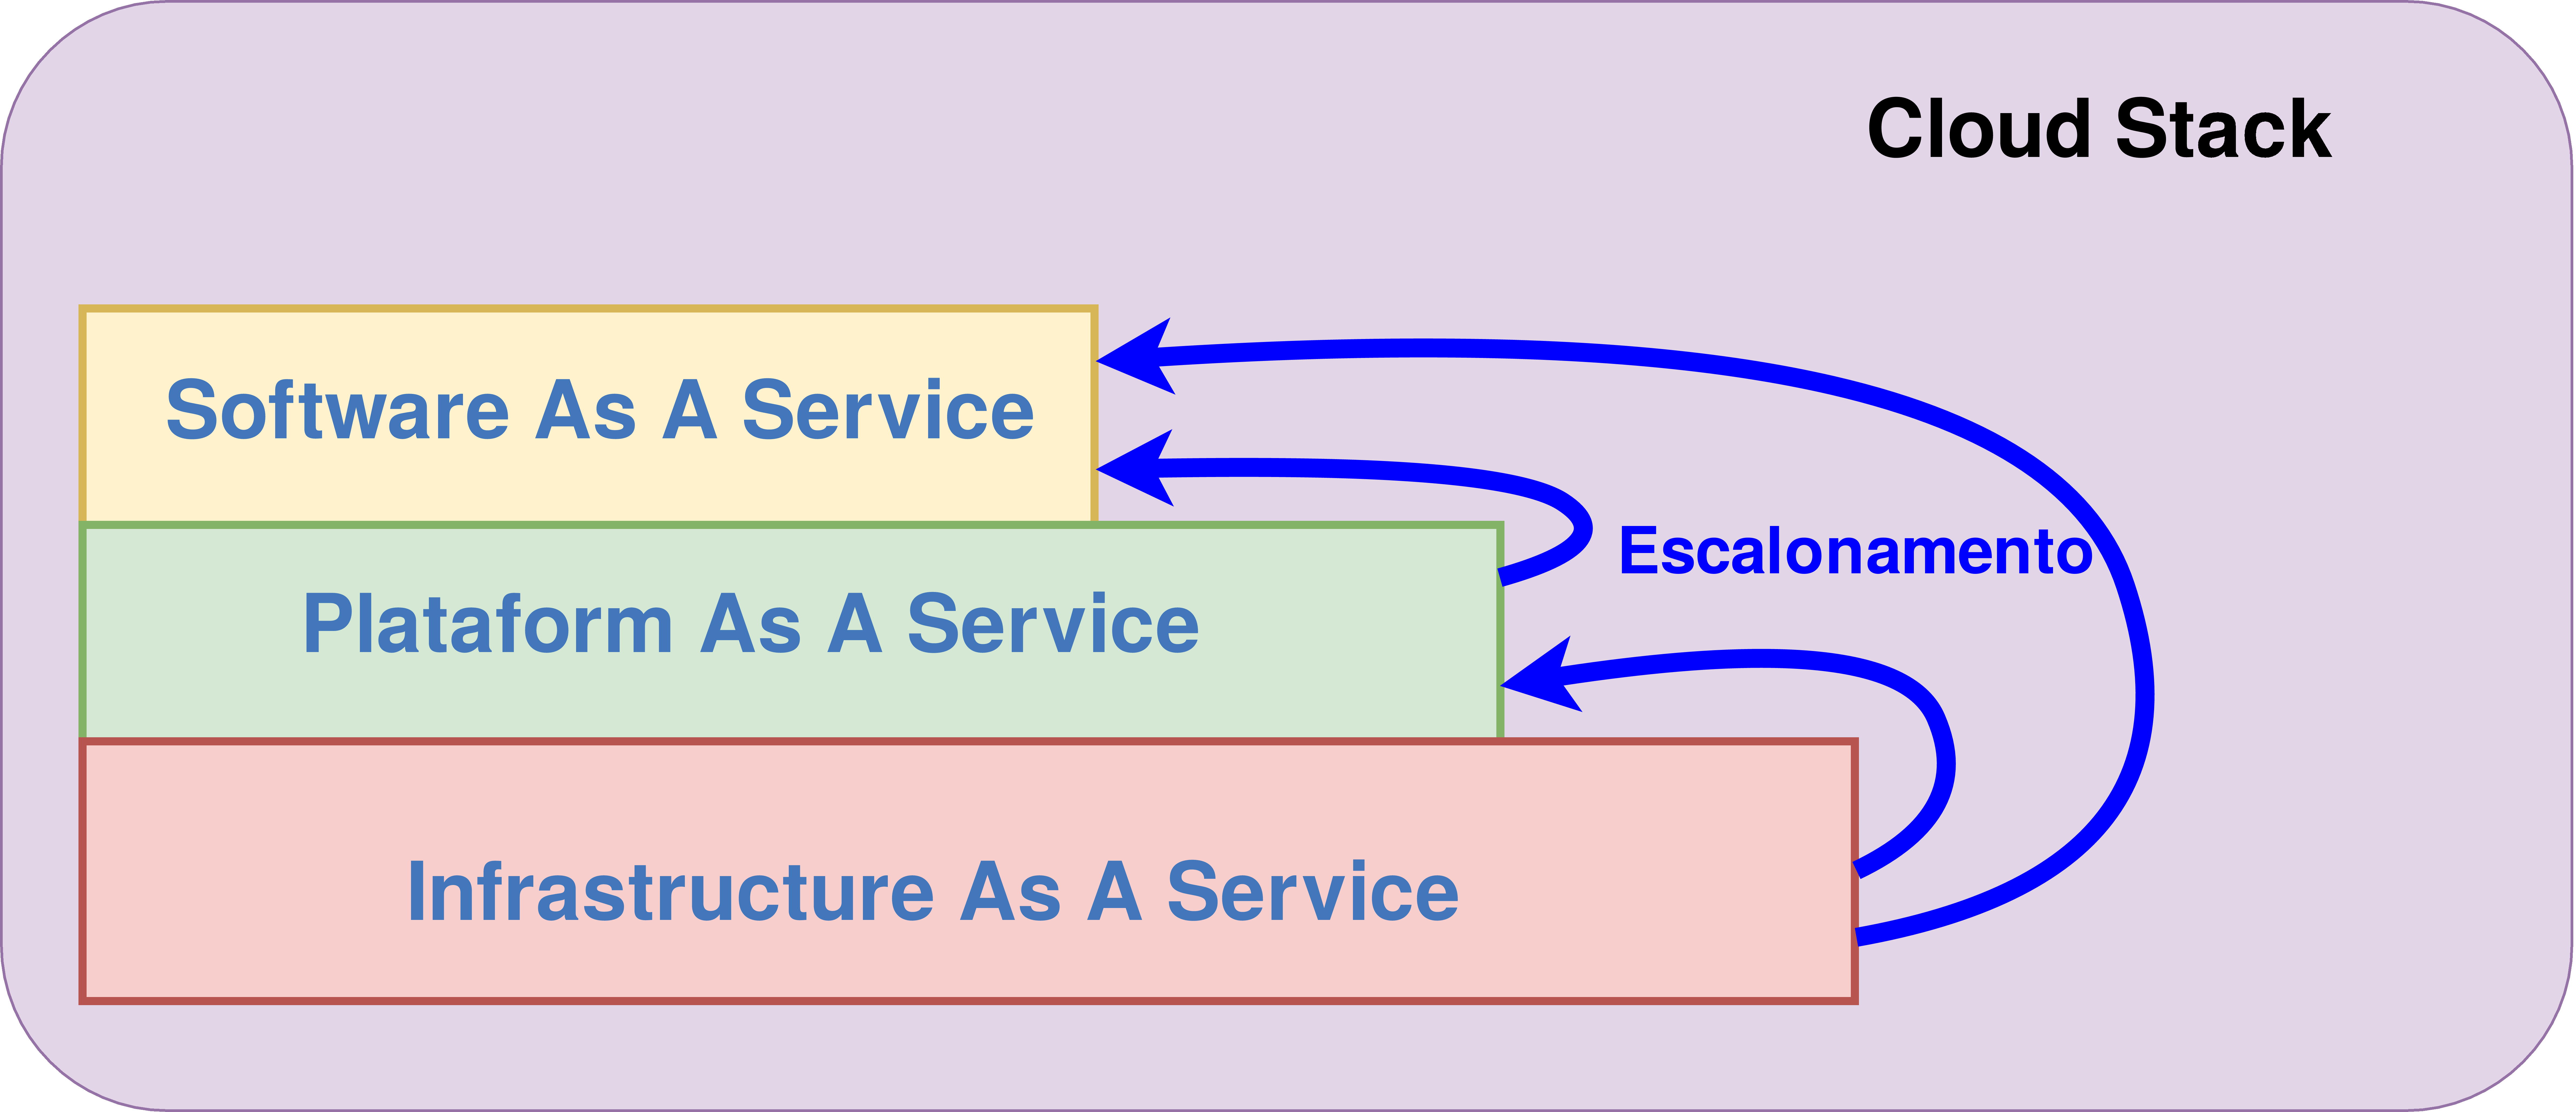
\includegraphics[width=15.0cm]{img/EscalonamentoStack.png}}
	\caption{Diferentes contextos em que o escalonamento pode acontecer na nuvem (adapatado de \cite{Zhan:2015:CCR:2775083.2788397}).}
	\label{EscalonamentoStack}
\end{figure}

Tendo a camada de aplicação como contexto, a atividade de escalonamento envolve aplicações de usuário, tarefas, e \textit{workflows} buscando otimizar eficiência do uso dos recursos físicos, podendo focar na garantia do \acrfull{QoS} contratado pelo usuário, em termos de performance, custo, confiabilidade entre outros aspectos, na eficiência do provedor, ou seja, otimizando o uso das máquinas com objetivo de melhorar o uso dos recursos computacionais para o provedor e escalonamento foca em negociação, ou seja, cujo foco é garantir o cumprimento de \acrfull{SLA}s, que são contratos de serviço entre o usuário do serviço e o provedor da nuvem \cite{Zhan:2015:CCR:2775083.2788397}.

Este trabalho focará no escalonamento em federações de nuvens computacionais. O qual recentemente presenciou a ascensão do uso de \acrfull{GPU} para processamento de propósito geral (\acrfull{GPGPU}\cite{Dimitrov:2009:USA:1513895.1513907}\cite{Yang:2010:GCM:1809028.1806606}. Nesse contexto, o problema do escalonamento pode ser formalmente definido como, dado:

\begin{itemize}
	\item Conjunto $T$ de tarefas;
	\item Conjunto $M$ de máquinas virtuais;
	\item Conjunto $C, |C| = |M|$ de CPUs das máquinas virtuais;
	\item Conjunto $G,  |G| \le |M|$ de GPUs das máquinas virtuais;
	\item Função $F: T \times (C \cup G) \to \mathbb{R}$, o qual estima o tempo de execução da tarefa $T_{i}$ no recurso designado.
\end{itemize}
Encontrar uma função injetora $A: T \to C \cup G$, que minimize $\sum_{t \in T} F(t, A(t) )$. Ou seja, buscar uma associação de tarefas para máquinas virtuais que minimize o tempo gasto para o processamento de todo o conjunto de tarefas.

Com base na taxonomia apresentar por Zhan \textit{et al.} \cite{Zhan:2015:CCR:2775083.2788397}, o problema de escalonamento abordado neste trabalho é considerado escalonamento com foco em federações parceiras na camada de infraestrutura. Outros tipos de escalonamento na camada de infraestrutura citados no mesmo trabalho são escalonamento para posicionamento do serviço, que busca delegar tarefas a locais próximos de onde o serviço foi solicitado, e o escalonamento focado em roteamento de dados, o qual busca alocar \acrshort{VM}s para uma tarefa descentralizada e forma a minimizar o gasto em comunicação entre as partes da aplicação.

\section{Trabalhos Relacionados}

Por mais que o problema do escalonamento seja um clássico na área da Ciência da Computação, são poucos que lidam com escalonamento em nuvens computacionais, e ainda menos os trabalhos que lidam com nuvens compostas por arquiteturas heterogêneas. 

Gouasmi \textit{et al.} \cite{MapReduce_sched_8034997} apresentam um algoritmo de \textit{MapReduce}\cite{Dean:2008:MSD:1327452.1327492} para escalonamento em nuvens federadas que foca em priorizar a execução de \textit{jobs} em nuvens/máquinas virtuais que já contém os dados necessários para a execução, com o objetivo de evitar transferências desnecessárias na rede. O algoritmo proposto é completamente distribuído e melhor do que o \textit{MapReduce} anteriormente utilizado, porém nada é dito sobre escalonamento para máquinas com arquiteturas heterogêneas.

Nguyen e Thoai \cite{7791859} propõem um sistema de intermediação para federações de nuvens horizontais, com foco na busca da melhor nuvem para auxiliar sobrecarga de serviços para execução. Levando em consideração que provedores de nuvens diferentes podem ter sua infraestrutura customizada com o objetivo de atender diferentes perfis de usuários que mais usam seus serviços, o algoritmo proposto leva em consideração tais características individuais de cada provedor. Novamente, nada é tratado sobre nuvens compostas por equipamentos com arquiteturas heterogêneas.

Jennings e Stadler \cite{Jennings:2015:RMC:2793474.2793493} documentaram  várias metodologias, utilizadas em diferentes contextos que o escalonamento ocorre em ambientes de nuvens computacionais, revelando detalhadamente muitos dos desafios enfrentados durante a concepção. Entretanto, nada é citado sobre federações de nuvens e os problemas de escalonamento enfrentados internamente num provedor de nuvem diferem dos enfrentados em ambientes de federação.

Kumrai \textit{et al.} \cite{7467407} trata, do escalonamento de tarefas do ponto de vista do intermediador, utilizando \acrfull{PSO}, que busca imitar um bando de pássaros. Cada elemento da população representa uma possível solução, que ao longo de interações tendem a encontrar o melhor resultado, baseado numa função que avalia quão bom cada elemento da população é. Também analisa uma variação multiobjetivo do \textit{Particle Swarm Optimization}, buscando solução boa tanto para o provedor de nuvem quanto para quem solicita o serviço. O problema do escalonamento apreciado neste artigo possui contexto similar ao que será enfrentado nesta monografia, entretanto, não é tratado o problema criado pelo uso de máquinas compostas por arquiteturas heterogêneas.

Mostageran \textit{et al.} \cite{7224588} documentam sobre intermediadores, conhecidos como \textit{brokers}, com foco em sua evolução para atenderem a níveis de qualidade de serviços propostos em \acrshort{SLA}s. Apresentando definições úteis para termos utilizados na área, como \textit{inter-cloud}, federação de nuvens e \textit{cloud broker}. É importante diferenciar os termos escalonador e intermediário. O intermediário mantém registro de entidades interessadas em um serviço e provedores desse serviço, incluindo busca de provedores e monitoramento das conexões feitas entre os interessados e os provedores. O escalonamento funciona em um escopo menor, que é gerenciar acesso a um recurso escasso buscando otimizar alguma métrica relativa ao seu contexto de uso, como por exemplo acesso de processos ao processador.

Diante dos trabalhos apresentados, nota-se que nenhum deles aborda o escalonamento para federações compostas por arquiteturas heterogêneas. Por isto, este trabalho propõe um escalonador para federações que utilizem equipamentos compostos por arquiteturas heterogêneas, o qual será apresentado na próxima seção.

\section{Escalonador Proposto para Plataformas de Federação}

O escalonador proposto para implementação segue a ideia básica de escalonamento de listas. Dessa forma, haverão três listas: lista de tarefas a serem executadas, lista de \acrshort{CPU}s disponíveis e lista de \acrshort{GPU}s disponíveis. O uso de listas para escalonamento é uma das abordagens principais para escalonamento, incluindo listas de listas\cite{MultilevelFQ}, pois é prático associar significados às posições na lista, por exemplo no Linux as posições 0 à 9 são utilizadas para \textit{threads} do sistema e de tempo real, enquanto as posições seguintes são usadas para \textit{threads} de usuário \cite{KernelsComp}.

A lista de tarefas é ordenada por tempo previsto de execução, que é dado por uma estimativa a partir do programa a ser executado e do arquivo de entrada. Essa ordenação será em ordem decrescente de tempo previsto, para que a tarefa que se estima como mais longa tenha alocada para si a melhor \acrshort{VM}. A lista de \acrshort{CPU}s disponíveis é ordenada com base na frequência e no número de núcleos. A lista de \acrshort{GPU}s tem sua ordem determinada pela quantidade de operações em pontos flutuante que consegue realizar por segundo. Dessa forma, o algoritmo proposto é detalhado no Algoritmo 1, e apresentado na forma de fluxo na Figura \ref{Escalonamento}.

%\newline
\begin{algorithm}
\caption{Escalonamento heterogêneo baseado em listas}
\begin{algorithmic}
	\Procedure{Escalonar}{listas lTarefas, lCPUs e lGPUs}
	\While{Existem tarefas que podem ser executadas nos recursos disponíveis?}
%		\State{$aux \gets lTarefas[0] $}
		\If{lTarefas[0] é capaz de executar em GPU}
			\If{$T_{previsto}(lGPUs[0]) < T_{previsto}(lCPUs[0])$}
			\State{Escalone\ lTarefas[0]\ para\ lGPUs[0]}
			\Else
				\State{Escalone\ lTarefas[0]\ para\ lCPUs[0]}
			\EndIf
		\Else
			\State{Escalone\ lTarefas[0]\ para\ lCPUs[0]}
		\EndIf
		\State{Remova a tarefa e o recurso alocado de suas respectivas listas.}
	\EndWhile
	\State{Encerra escalonamento}
\EndProcedure
\end{algorithmic}
\end{algorithm}

O escalonamento busca associar as tarefas mais longas às máquinas com maior capacidade de processamento, sendo que, para cada tarefa, é analisado se vale a pena alocar a tarefa em uma \acrshort{VM} que possua \acrshort{GPU}.


\begin{figure}[htbp]
%	\centerline{\includegraphics[scale=0.04]{img/EscalonadorProposto.png}}
	\centerline{\includegraphics[scale=0.032]{img/EscalonadorProposto2.png}}
	\caption{Diagrama de Funcionamento do Algoritmo de Escalonamento Proposto.}
	\label{Escalonamento}
\end{figure}


Assim sendo, observe que para o algoritmo mostrado na Figura \ref{Escalonamento} ser válido, pressupõe-se que toda tarefa do algoritmo é capaz de executar em \acrshort{CPU}. O pressuposto simplifica o primeiro passo do algoritmo, exibido na Figura \ref{Escalonamento}, pois se a lista de \acrshort{CPU}s não estiver vazia, essa condição é automaticamente satisfeita.

Dessa forma, sob a ótica do trabalho de Casavant e Kuhl \cite{4634_TaxonomiaEscalonador}, o algoritmo desenvolvido neste trabalho pode ser classificado como global, estático, sub-ótimo e aproximado.%, utilizando teoria das filas.

Escalonamento local é o responsável por decidir a execução de processos a \textit{time-slices} de um processador, o escalonador desenvolvido neste trabalho, opera no nível de decidir quais processos serão executados em quais máquinas virtuais, deixando o escalonamento local a cargo do sistema operacional da máquina em questão.

Casavant e Kuhl \cite{4634_TaxonomiaEscalonador} definem como escalonamento estático, o escalonamento no qual é conhecido durante a inicialização de uma máquina, que \textit{jobs} ela executará. Esta condição é satisfeita, pois um \textit{workflow} precisa ser bem definido para ser executado no BioNimbuZ. Vale a pena ressaltar que o escalonamento estático também pode ser denominado escalonamento determinístico.

O escalonador desenvolvido neste trabalho é considerado sub-ótimo e aproximado, porque nem todas as informações sobre os \textit{jobs} de um \textit{workflow} são conhecidas, o BioNimbuZ possui o Serviço de Predição para estimar o tempo de execução de um \textit{job}, e por isso este escalonador é considerado aproximado.


O próximo capítulo apresentará os desafios enfrentados na implementação e implantação do escalonador na plataforma BioNimbuZ.
%O próximo capítulo apresentará o BioNimbuZ, a plataforma de federação de nuvem selecionada para a implementação de algoritmo, também serão apresentados informação sobre a implementação do escalonador.



%Colocar aqui como testar o escalonador??

